\documentclass{article}
\usepackage{amsmath, amssymb, ctex, graphicx, color}
\usepackage[margin=1in]{geometry}
\usepackage{setspace} % 行距控制
\usepackage{array}
\usepackage{makecell}
\usepackage{booktabs}

\usepackage{algorithm}
\usepackage{algpseudocode}
\usepackage{xcolor}
% 把默认注释符号 ▷ 改成行尾 // 等宽紫色，并右对齐
\renewcommand{\algorithmiccomment}[1]{\hfill\texttt{\textcolor{violet}{// #1}}}
% 定义 Input / Output 关键字（默认是 Require / Ensure）
\algnewcommand\algorithmicinput{\textbf{Input:}}
\algnewcommand\algorithmicoutput{\textbf{Output:}}
\algnewcommand\Input{\item[\algorithmicinput]}
\algnewcommand\Output{\item[\algorithmicoutput]}

\usepackage{titling}\setlength{\droptitle}{-2cm} 
\title{Ch8. Backpropagation \hfill 第8章 反向传播 \\ 
Section 8.1. Evaluation of Gradients \hfill 第8.1节 梯度计算 \\ 
8.1.5. The Jacobian matrix \hfill 8.1.5. 雅可比矩阵 }
\author{《深度学习基础》课程小组}
% \date{}
 
\begin{document}
\maketitle
% \tableofcontents

\setlength{\parindent}{0pt} % 取消首行缩进
\setlength{\parskip}{1.5em} % 设置段落之间的距离

\noindent\rule{\linewidth}{0.4pt}

\section{P1 8.1.5 The Jacobian matrix}

We have seen how \underline{the derivatives of an error function with respect to the weights} can be obtained by propagating errors backwards through the network. 

Backpropagation can also be used to calculate other derivatives. 

Here we consider the evaluation of the \textbf{Jacobian matrix}, whose elements are given by the derivatives of the network outputs with respect to the inputs:
\begin{equation}
    J_{ki} \equiv \frac{\partial y_k}{\partial x_i}
    \tag{8.26}
\end{equation}
where each such derivative is evaluated with all other inputs held fixed. 

Jacobian matrices play a useful role in systems built from a number of distinct modules, as illustrated in Figure~8.3. 

Each module can comprise a fixed or learnable function, which can be linear or nonlinear, so long as it is differentiable.

{\color{red}
翻译：

我们已经了解了如何通过在网络中反向传播误差来获得\underline{误差函数关于权重的导数}。

反向传播也可以用于计算其他的导数。

在这里，我们考虑\textbf{雅可比矩阵}（Jacobian matrix）的求值，其元素由网络输出关于输入的导数给出：
\begin{equation}
    J_{ki} \equiv \frac{\partial y_k}{\partial x_i}
    \tag{8.26}
\end{equation}
其中，每个这样的导数都是在保持所有其他输入固定的情况下计算的。

雅可比矩阵在由多个不同模块构建的系统中发挥着重要作用，如图~8.3 所示。

每个模块可以包含一个固定的或可学习的函数，该函数可以是线性的或非线性的，只要它是可微的即可。
}

{\color{blue}
\underline{问：为什么要计算输出变量关于输入变量的雅可比矩阵？}

答：计算输出变量关于输入变量的雅可比矩阵，其核心目的是量化神经网络对输入扰动的局部敏感性，并作为连接网络内部结构与外部行为的关键数学桥梁。它不仅是理论分析的工具，更是实现模型优化、误差传播和系统集成的基础。

1. 衡量模型对输入变化的敏感度

雅可比矩阵的每个元素 $J_{ki} = \partial y_k / \partial x_i$ 表示第 $k$ 个输出对第 $i$ 个输入的瞬时变化率。这意味着：\\ 
若某个 $J_{ki}$ 值很大，说明输出 $y_k$ 对输入 $x_i$ 的微小变动非常敏感；\\
若 $J_{ki}$ 接近零，则说明该输入对当前输出几乎无影响。

这种敏感性分析在以下场景中至关重要：\\
特征重要性评估：识别哪些输入特征对模型输出贡献最大；\\
对抗样本防御：理解模型在哪些输入方向上容易被欺骗；\\
模型解释性：为“黑箱”模型提供局部可解释的梯度依据。

2. 支持模块化系统中的误差传播

正如文中提到，雅可比矩阵在由多个模块组成的系统中扮演关键角色。当系统由多个可微子模块串联或并联构成时，整个系统的输出对输入的导数可以通过各模块的雅可比矩阵相乘得到。这使得：

误差可以逐模块反向传播：即使某个模块是固定的（如预训练的特征提取器），只要它是可微的，就可以通过雅可比矩阵将最终误差“传递”回前面的模块；

支持端到端训练：即使部分模块不可学习，只要可微，就能参与梯度计算，从而实现联合优化。

3. 用于近似输出变化与不确定性传播

在实际应用中，我们常常需要估计输入的小扰动 $\Delta x_i$ 会导致输出多大的变化 $\Delta y_k$。根据一阶泰勒展开，有：
$$
\Delta y_k \approx \sum_i J_{ki} \Delta x_i
$$
这个线性近似在以下场景中非常有用：\\
输入噪声传播分析：评估传感器噪声或数据预处理误差对最终预测的影响；\\
模型鲁棒性评估：判断模型在输入扰动下是否稳定；\\
实时控制系统：在控制理论中，雅可比矩阵常用于线性化非线性系统，以便设计控制器。

4. 作为高阶导数计算的基础

雅可比矩阵是计算海森矩阵（Hessian Matrix）等高阶导数的前置步骤。例如，在优化算法中，海森矩阵描述了损失函数的曲率，而它的计算往往依赖于雅可比矩阵的乘积。此外，在某些贝叶斯推断方法中，雅可比矩阵也用于计算后验分布的协方差结构。
}

\noindent\rule{\linewidth}{0.4pt}

\section{P2}

Suppose we wish to minimize an error function $E$ with respect to the parameter $w$ in Figure~8.3. 

The derivative of the error function is given by
\begin{equation}
    \frac{\partial E}{\partial w} = \sum_{k,j} \frac{\partial E}{\partial y_k} \frac{\partial y_k}{\partial z_j} \frac{\partial z_j}{\partial w}
    \tag{8.27}
\end{equation}
in which the Jacobian matrix for the red module in Figure~8.3 appears as the middle term on the right-hand side.

Figure 8.3 Caption: Illustration of a modular deep learning architecture in which the Jacobian matrix can be used to backpropagate error signals from the outputs through to earlier modules in the system.

\begin{figure}[htbp]
    \centering
    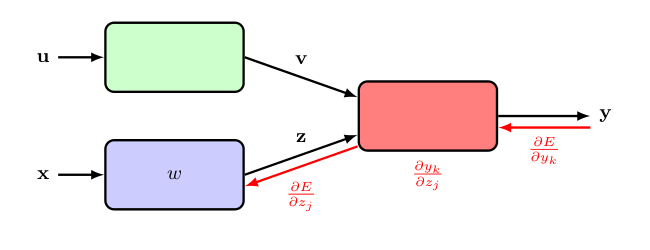
\includegraphics[width=0.5\textwidth]{figure-8-3.png}
    \caption{图8-3：右边的红色模块是雅可比矩阵}
    % \label{}
\end{figure}

\noindent\rule{\linewidth}{0.4pt}

{\color{red}
翻译：

假设我们希望针对图~8.3 中的参数 $w$ 来最小化误差函数 $E$。

该误差函数的导数由下式给出：
\begin{equation}
    \frac{\partial E}{\partial w} = \sum_{k,j} \frac{\partial E}{\partial y_k} \frac{\partial y_k}{\partial z_j} \frac{\partial z_j}{\partial w}
    \tag{8.27}
\end{equation}
其中，图~8.3 中红色模块的雅可比矩阵即为等式右侧的中间项。

图 8.3 图注：模块化深度学习架构示意图。在该架构中，雅可比矩阵可用于将误差信号从输出端反向传播至系统中的早期模块。
}

\section{P3}

Because the Jacobian matrix provides a measure of the local sensitivity of the outputs to changes in each of the input variables, it also allows known errors $\Delta x_i$ associated with the inputs to be propagated through the trained network to estimate their contribution $\Delta y_k$ to the errors at the outputs, through the relation
\begin{equation}
    \Delta y_k \approx \sum_i \frac{\partial y_k}{\partial x_i} \Delta x_i
    \tag{8.28}
\end{equation}
which assumes that the $|\Delta x_i|$ are small. 

In general, the network mapping represented by a trained neural network will be nonlinear, and so the elements of the Jacobian matrix will not be constants but will depend on the particular input vector used. 

Thus, (8.28) is valid only for small perturbations of the inputs, and the Jacobian itself must be re-evaluated at each new input vector.

{\color{red}
翻译：

由于雅可比矩阵能够衡量输出对各个输入变量变化的局部敏感度，因此它也允许将与输入相关的已知误差 $\Delta x_i$ 通过训练好的网络进行传播，从而估计它们对输出端误差的贡献 $\Delta y_k$。这一估计通过以下关系式实现：
\begin{equation}
    \Delta y_k \approx \sum_i \frac{\partial y_k}{\partial x_i} \Delta x_i
    \tag{8.28}
\end{equation}
该关系式的前提假设是 $|\Delta x_i|$ 的值足够小。

通常情况下，由训练好的神经网络所表示的网络映射是非线性的，因此雅可比矩阵的元素并非恒定常数，而是取决于所使用的特定输入向量。

因此，公式 (8.28) 仅在输入发生微小扰动时有效，并且对于每一个新的输入向量，都必须重新计算雅可比矩阵。

% 这部分和对抗样本攻击（比如FGSM）直接相关。
}

\noindent\rule{\linewidth}{0.4pt}

\section{P4}

The Jacobian matrix can be evaluated using a backpropagation procedure that is like the one derived earlier for evaluating the derivatives of an error function with respect to the weights. 

We start by writing the element $J_{ki}$ in the form
\begin{equation}
    J_{ki} \equiv \frac{\partial y_k}{\partial x_i} = \sum_j \frac{\partial y_k}{\partial a_j} \frac{\partial a_j}{\partial x_i} = \sum_j w_{ji} \frac{\partial y_k}{\partial a_j}
    \tag{8.29}
\end{equation}
where we have made use of (8.5). 

The sum in (8.29) runs over all units $j$ to which the input unit $i$ sends connections (for example, over all units in the first hidden layer in the layered topology considered earlier). 

We now write down a recursive backpropagation formula for the derivatives $\partial y_k / \partial a_j$:
\begin{equation}
    \frac{\partial y_k}{\partial a_j} = \sum_\ell \frac{\partial y_k}{\partial a_\ell} \frac{\partial a_\ell}{\partial z_j} = h'(a_j) \sum_\ell w_{\ell j} \frac{\partial y_k}{\partial a_\ell}
    \tag{8.30}
\end{equation}
where the sums run over all units $\ell$ to which unit $j$ sends connections (corresponding to the first index of $w_{\ell j}$). 

Again, we have made use of (8.5) and (8.6). 

This backpropagation starts at the output units, for which the required derivatives can be found directly from the functional form of the output-unit activation function. 

{\color{red}
翻译：

雅可比矩阵可以使用类似于前文推导的、用于计算误差函数关于权重导数的反向传播过程来进行计算。

我们首先将元素 $J_{ki}$ 写成如下形式：
\begin{equation}
    J_{ki} \equiv \frac{\partial y_k}{\partial x_i} = \sum_j \frac{\partial y_k}{\partial a_j} \frac{\partial a_j}{\partial x_i} = \sum_j w_{ji} \frac{\partial y_k}{\partial a_j}
    \tag{8.29}
\end{equation}
在此我们利用了公式 (8.5)。

公式 (8.29) 中的求和遍历了所有接收来自输入单元 $i$ 连接的单元 $j$（例如，在前文考虑的分层拓扑结构中，遍历第一隐藏层中的所有单元）。

接下来，我们为导数 $\partial y_k / \partial a_j$ 写出一个递归的反向传播公式：
\begin{equation}
    \frac{\partial y_k}{\partial a_j} = \sum_\ell \frac{\partial y_k}{\partial a_\ell} \frac{\partial a_\ell}{\partial z_j} = h'(a_j) \sum_\ell w_{\ell j} \frac{\partial y_k}{\partial a_\ell}
    \tag{8.30}
\end{equation}
其中，求和遍历了所有接收来自单元 $j$ 连接的单元 $\ell$（对应于 $w_{\ell j}$ 的第一个下标）。

同样地，我们利用了公式 (8.5) 和 (8.6)。

该反向传播过程从输出单元开始，对于输出单元，所需的导数可以直接从其激活函数的解析形式中得出。
}

\noindent\rule{\linewidth}{0.4pt}

\section{P5}

For linear output units, we have
\begin{equation}
    \frac{\partial y_k}{\partial a_\ell} = \delta_{k\ell}
    \tag{8.31}
\end{equation}
where $\delta_{k\ell}$ are the elements of the identity matrix and are defined by
\begin{equation}
    \delta_{k\ell} =
    \begin{cases}
        1, & \text{if } k = \ell, \\
        0, & \text{otherwise}.
    \end{cases}
    \tag{8.32}
\end{equation}

If we have individual logistic sigmoid activation functions at each output unit, then
\begin{equation}
    \frac{\partial y_k}{\partial a_\ell} = \delta_{k\ell} \sigma'(a_k)
    \tag{8.33}
\end{equation}
whereas for softmax outputs, we have
\begin{equation}
    \frac{\partial y_k}{\partial a_\ell} = \delta_{k\ell} y_\ell - y_k y_\ell.
    \tag{8.34}
\end{equation}

{\color{red}
翻译+注释：

对于线性输出单元，【因为 $y_k=a_k$, 即激活函数是恒等函数，】我们有：
\begin{equation}
    \frac{\partial y_k}{\partial a_\ell} = \delta_{k\ell}
    \tag{8.31}
\end{equation}
其中 $\delta_{k\ell}$ 是单位矩阵的元素，其定义为：
\begin{equation}
    \delta_{k\ell} =
    \begin{cases}
        1, & \text{若 } k = \ell, \\
        0, & \text{其他情况}.
    \end{cases}
    \tag{8.32}
\end{equation}

如果每个输出单元都使用独立的逻辑 Sigmoid 激活函数，则有：
\begin{equation}
    \frac{\partial y_k}{\partial a_\ell} = \delta_{k\ell} \sigma'(a_k)
    \tag{8.33}
\end{equation}
注释：独立是说$y_k$仅与$a_k$有关，与其它$a_{\ell}$无关，逻辑激活函数是 
$$
y_k=\sigma(a_k)=\frac{1}{1+\exp(-a_k)}=\frac{\exp(a_k)}{\exp(a_k)+1}.
$$

而对于 Softmax 输出，我们有：
\begin{equation}
    \frac{\partial y_k}{\partial a_\ell} = \delta_{k\ell} y_\ell - y_k y_\ell.
    \tag{8.34}
\end{equation}
注释：这个 Softmax 激活函数是
$$
y_k = \frac{\exp(a_k)}{\sum\limits_\ell\exp(a_\ell)}.
$$
分情况 $k=\ell$ 与 $k\neq \ell$ 可以验证上式。

}

\noindent\rule{\linewidth}{0.4pt}

\section{P6}

We can summarize the procedure for calculating the Jacobian matrix as follows. 

Apply the input vector corresponding to the point in input space at which the Jacobian matrix is to be evaluated, and forward propagate in the usual way to obtain the states of all the hidden and output units in the network. 

Next, for each row $k$ of the Jacobian matrix, corresponding to the output unit $k$, backpropagate using the recursive relation (8.30), starting with (8.31), (8.33) or (8.34), for all the hidden units in the network. 

Finally, use (8.29) for the backpropagation to the inputs. 

The Jacobian can also be evaluated using an alternative \textit{forward propagation} formalism, which can be derived in an analogous way to the backpropagation approach given here.

{\color{red}
翻译：

我们可以将计算雅可比矩阵的过程总结如下。

首先，输入对应于输入空间中待求雅可比矩阵的点的输入向量，并以常规方式进行前向传播，从而获取网络中所有隐藏单元和输出单元的状态。

接下来，对于雅可比矩阵的每一行 $k$（对应于输出单元 $k$），利用递归关系式 (8.30) 进行反向传播，并以 (8.31)、(8.33) 或 (8.34) 作为起点，遍历网络中的所有隐藏单元。

最后，利用 (8.29) 将反向传播继续至输入层。

此外，雅可比矩阵也可以采用另一种\textit{前向传播}（forward propagation）形式来计算，其推导方式与本文给出的反向传播方法类似。
}

{\color{blue}
\underline{习题8.5：如何用前向传播方法计算雅可比矩阵？}

答：反向传播是“从后往前”算导数，而前向传播是“从前往后”同时计算数值和导数。

核心概念：前向模式自动微分

在神经网络中，我们通常关心的是损失函数对权重的梯度（标量对标量或向量），这时反向传播效率最高。但是，当我们需要计算输出对输入的导数（即雅可比矩阵 $J_{ki} = \partial y_k / \partial x_i$）时，情况就不同了。

反向传播（Backpropagation）：适合输出维度小、输入维度大的情况。它一次只能计算一个输出对所有输入的梯度。

前向传播（Forward Propagation）：适合输入维度小、输出维度大的情况。它一次可以计算所有输出对某一个输入的梯度。

具体推导逻辑：Bishop 书中提到的“analogous way”是指利用链式法则，但方向相反。

定义变量：假设网络中第 $j$ 个单元的激活值为 $z_j$，加权输入为 $a_j$。在前向传播中，我们不仅计算 $z_j$ 的值，还同时计算它对某个特定输入 $x_i$ 的偏导数 $\frac{\partial z_j}{\partial x_i}$。

递归公式：对于隐藏层单元 $j$，其加权输入 $a_j$ 由\underline{前一层的输出 $z_\ell$} 线性组合而成：
$$ a_j = \sum_\ell w_{j\ell} z_\ell $$
根据链式法则，对输入 $x_i$ 求导：
$$ \frac{\partial a_j}{\partial x_i} = \sum_\ell w_{j\ell} \frac{\partial z_\ell}{\partial x_i} $$
接着，经过激活函数 $h(\cdot)$ 得到 $z_j = h(a_j)$，其导数为：
$$ \frac{\partial z_j}{\partial x_i} = h'(a_j) \frac{\partial a_j}{\partial x_i} 
= h'(a_j) \sum_\ell w_{j\ell} \frac{\partial z_\ell}{\partial x_i} 
$$

算法流程

1. 初始化：对于输入层，$\frac{\partial x_k}{\partial x_i} = \delta_{ki}$（克罗内克 $\delta$ 函数，即自己对自己的导数是1，其他是0）。

2. 前向传递：按照网络的层级顺序，从输入层向输出层逐层计算。每一层都利用上一层的导数结果，乘以权重和激活函数的导数，得到当前层的导数。

3. 输出：最终到达输出层时，我们就得到了所有输出 $y_k$ 对特定输入 $x_i$ 的导数 $\frac{\partial y_k}{\partial x_i}$。这正好构成了雅可比矩阵的一列。

总结：Bishop 这句话的意思是：计算雅可比矩阵不只有“反向传播”这一条路。我们可以模仿反向传播的链式法则逻辑，但是从输入端开始，顺着网络流向输出端，一边计算神经元数值，一边计算导数。这种方法在数学上完全等价，只是在不同的维度配置下计算效率不同。
}

\noindent\rule{\linewidth}{0.4pt}

\section{P7}

Again, the implementation of such algorithms can be checked using numerical differentiation in the form
\begin{equation}
    \frac{\partial y_k}{\partial x_i} = \frac{y_k(x_i + \epsilon) - y_k(x_i - \epsilon)}{2\epsilon} + \mathcal{O}(\epsilon^2),
    \tag{8.35}
\end{equation}
which involves $2D$ forward propagation passes for a network having $D$ inputs and therefore requires $\mathcal{O}(DW)$ steps in total.

{\color{red}
翻译：

同样地，此类算法的实现可以通过如下形式的数值微分来进行检验：
\begin{equation}
    \frac{\partial y_k}{\partial x_i} = \frac{y_k(x_i + \epsilon) - y_k(x_i - \epsilon)}{2\epsilon} + \mathcal{O}(\epsilon^2),
    \tag{8.35}
\end{equation}
对于一个具有 $D$ 个输入的网络，该方法需要进行 $2D$ 次前向传播，因此总共需要 $\mathcal{O}(DW)$ 的计算步数。
}

{\color{blue}
\underline{问：为什么总共需要 $\mathcal{O}(DW)$ 的计算步数？}

答：这个计算复杂度 $\mathcal{O}(DW)$ 是由数值微分的采样次数与单次前向传播的计算成本相乘得来的。我们可以将其拆解为以下两个部分来理解：

1. 为什么需要 $2D$ 次前向传播？

公式 (8.35) 使用的是中心差分法（Central Difference）来近似偏导数：
$$ \frac{\partial y_k}{\partial x_i} \approx \frac{y_k(x_i + \epsilon) - y_k(x_i - \epsilon)}{2\epsilon} $$

$D$ 的含义：网络有 $D$ 个输入变量（$x_1, x_2, ..., x_D$）。

计算偏导数的过程：为了求出对某一个特定输入 $x_i$ 的偏导数，我们需要计算两次网络输出：一次是 $x_i$ 加上 $\epsilon$，另一次是 $x_i$ 减去 $\epsilon$。因此，计算一个输入的偏导数需要 2 次前向传播。

计算雅可比矩阵：雅可比矩阵包含所有 $D$ 个输入的偏导数。因此，总共需要进行 $2 \times D$ 次前向传播。

2. 为什么每次前向传播需要 $\mathcal{O}(W)$ 步？

$W$ 的含义：$W$ 是神经网络中权重（weights）和偏置（biases）的总数。

前向传播的本质：神经网络的前向传播本质上是一系列矩阵乘法和激活函数的运算。在一个全连接网络中，每一层的计算量与该层的权重数量成正比。

整体复杂度：从输入层到输出层，网络需要遍历并计算所有的权重和偏置。因此，完成一次完整的前向传播，其计算步数与网络参数总量 $W$ 成正比，即时间复杂度为 $\mathcal{O}(W)$。

3. 综合得出 $\mathcal{O}(DW)$

将上述两者结合：
$$ \text{总计算步数} = (\text{前向传播次数}) \times (\text{单次前向传播的计算步数}) $$
$$ \text{总计算步数} = (2D) \times \mathcal{O}(W) = \mathcal{O}(DW) $$

直观对比：这就是为什么在实际工程中，我们通常不会用数值微分来训练神经网络或计算雅可比矩阵。如果网络有 10,000 个输入（$D=10000$）和 1,000,000 个参数（$W=10^6$），用数值微分计算一次雅可比矩阵需要 $2 \times 10^{10}$ 步运算，这在计算上是完全不可行的。而利用前文提到的反向传播算法，计算完整的雅可比矩阵只需要大约 $\mathcal{O}(W)$ 到 $\mathcal{O}(KW)$ 的步数（$K$ 为输出维度），效率高了几个数量级。

% 前面提到数值微分效率低，但它的优势在于简单可靠，可以用来验证反向传播的实现是否正确。需要我帮你写一段 Python 代码，演示如何用数值微分验证反向传播的梯度计算吗？

}

\end{document}
